\chapter{A New Recruit}

% Une partie destinée à un nouvel arrivant dans la société qui va reprendre / poursuivre le projet dans lequel vous avez été impliqué. Il faut donc lui décrire le contexte de l’entreprise, du projet, l’architecture générale de celui-ci, le contexte et l’organisation de l’équipe de travail, le tout de façon synthétique. Il faudra également y apporter les précisions quant aux difficultés rencontrées dans le projet.

This part has for objective to onboard a new recruit in a project that I worked on during my internship which is \gls{san-iscsi-csi}, developped as an \glsdef{open-source} software on \glsdef{github}. This software allows to perform \glsdef{dynamic-volume-provisioning} on \glsdef{k8s} and \glsdeff{\acrshort}{csi}-compliant \glsdeff{\glspl}{k8s-co}.

\clearpage

\section{Introduction}

In order to onboard you on our project \gls{san-iscsi-csi}, we will review some information you should know about it and about the company \gls{enix} more generally.

We will first discuss the company context, followed by the project context and its general architecture and finally describe the context and organisation of the project work team.

\section{Company context}

\gls{enix} SAS is a company selling \glsdef{cloud}, \glsdef{devops} and \glsdef{k8s} services in a \glsdeff{\acrshort}{b2b} business model. The company has been created in the early 2000s in the LAN parties environment. Sébastien, Romain, Alexandre, Jérôme and Laurent, student then, started this company in response to needs in infrastructure and networking during those events.

Today, \gls{enix} counts 15 employees and a few external collaborators. We work for some big clients like \gls{xbto}, \gls{tdf}, \gls{maif}, \gls{ulule}, \gls{airbus} and others.

\section{Project context}

The idea from which \gls{san-iscsi-csi} came from is the one to implement all cutting-edge features of \glsdef{k8s} in terms of storage, using storage appliances initially not intended for this purpose. It targets mainly \glsdef{on-prem} \glsdef{cloud} infrastructures.

\subsection{Cloud context}

Nowadays, \glsdef{containerization} (see \figref{fig:containers}) of applications has become a golden standard in the industry. It allows to build, ship and run applications anywhere \glsdef{on-prem} or in the \glsdef{cloud}, with particular focus on portability and operability. \glsdeff{\glspl}{container} allow to run softwares in a sandboxed environment, which increase security and are lighter than \glsdeff{\glspl}{virtual-machine} which require a full \glsdeff{\acrshort}{os} running for each instances.

\begin{figure}[h]
    \centering
    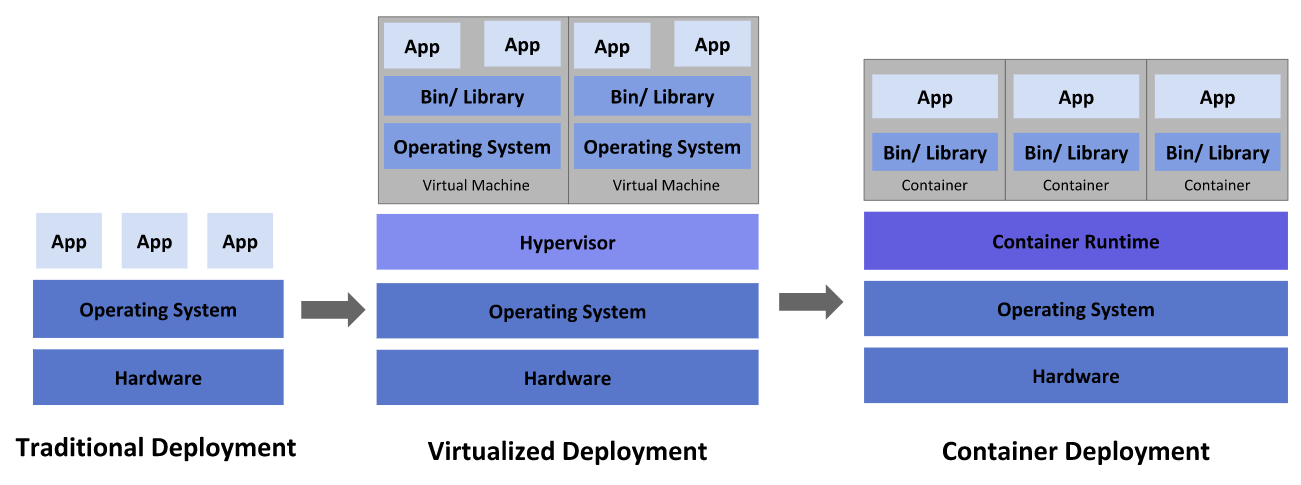
\includegraphics[width=\textwidth]{schema-containers.png}
    \caption{From traditional to containerized deployments}
    \label{fig:containers}
\end{figure}

A solution like \glsdef{k8s} is used to orchestrate \glsdeff{\glspl}{container} and is able to manage the whole underlying infrastructure (network, storage, databases, etc...). It is composed of several specialized services that operate a set of \glsdeff{\glspl}{container} in the right conditions.

As shown in \figref{fig:k8s-components}, there is on one hand the control plane, which control the state of the \glsdef{cluster}, and on the other hand \glsdef{k8s} nodes, which are servers running orchestrated \glsdeff{\glspl}{container}.

\begin{figure}[h]
    \centering
    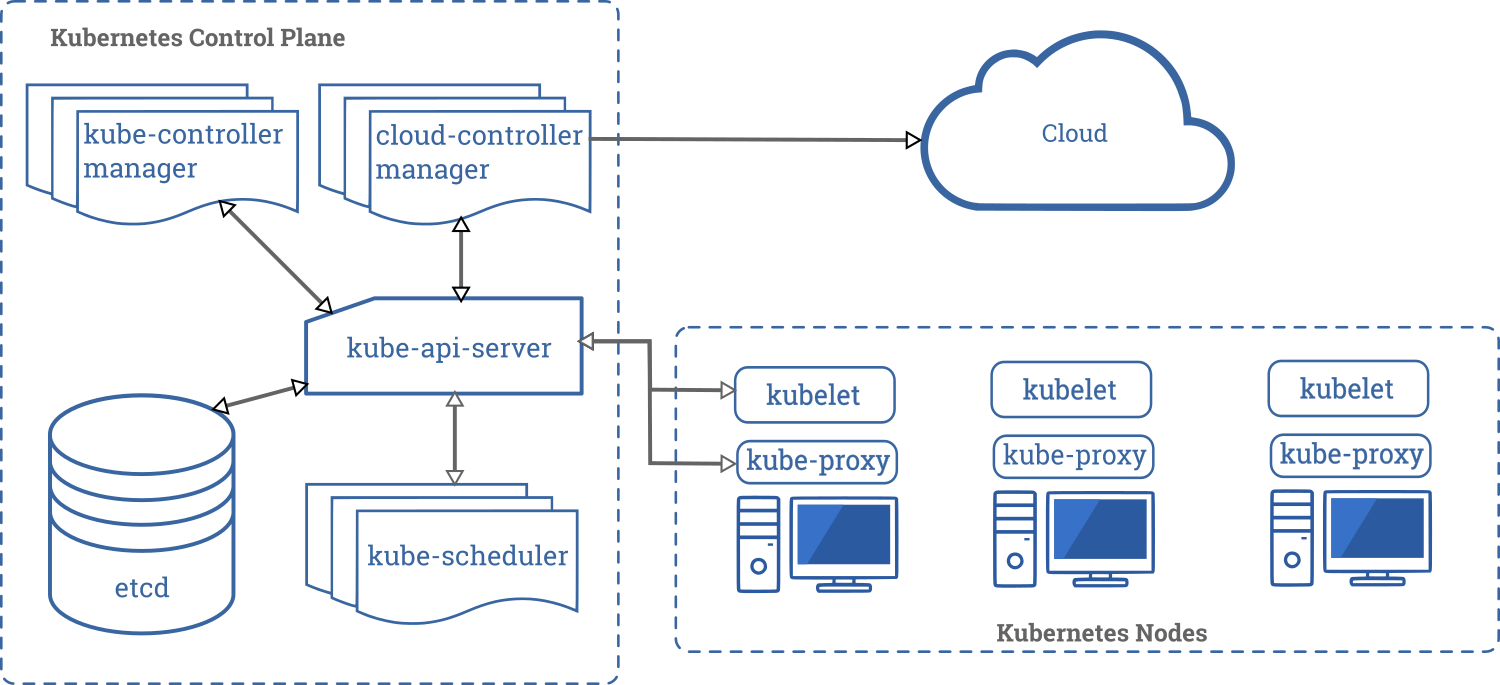
\includegraphics[width=\textwidth]{schema-kubernetes-components.png}
    \caption{Kubernetes components}
    \label{fig:k8s-components}
\end{figure}

On the storage side comes the concept of \glsdef{volume}, which is actually a storage unit. A volume can be persistant or not, local or distant, dynamically or statically provisioned. Statically means that the \glsdef{volume} has been provisioned by someone manually, whereas dynamically means that someone only asked to have a \glsdef{volume} available and some software got the work done.

\glsdef{csi} is a standard that comes to unify the process of \glsdef{dynamic-volume-provisioning} across \glsdeff{\glspl}{k8s-co}. It allows to dynamically provisionning of \glsdef{k8s-pv} through a configuration object called \glsdef{k8s-pvc}.

\subsection{Typical storage solution}

\color{darkgreen}
La société Dot Hill Systems Corp construit depuis 1997 des baies de stockage bon marché, elle a été rachetée par Seagate en 2015.

Les modèles de baies disponibles depuis quelques années possèdent les fonctionnalités typiques attendues tout en restant bon marché. Elles sont d'ailleurs rebadgées par plusieurs constructeurs : Dell, HP, ...

La fonctionnalité qui nous intéresse en particulier dans le cadre du projet Dothill-CSI est la disponibilité d'une API (documentée) permettant de contrôler la baie en question.
\color{black}

\subsection{Technical opportinity}

\color{darkgreen}
Kubernetes permet de gérer le stockage persistant attaché aux conteneurs via des ressources appelées Persistent Volumes. L'état de l'art étant de mettre à disposition à la volée des volumes en fonction de la demande, via le principe de Dynamic Volume Provisioning.

La liste des types de volumes supportés est conséquente https://kubernetes.io/docs/concepts/storage/volumes/\#types-of-volumes. Elle intègre notamement le protocole iSCSI qui est supporté par les baies de stockage DotHill. Mais ce protocole iSCSI ne permet pas nativement le provisioning des volumes. C'est ce besoin précis que le projet Dothill-CSI cherche à traiter.
\color{black}

\section{General project architecture}

\subsection{Working principle}

\color{darkgreen}
L'API Kubernetes propose deux ressources correspondant respectivement à une « demande de stockage » (Persistent Volume Claim) et à du « stockage disponible » (Persistent Volume). Les applications ayant besoin de stockage vont créer un ou plusieurs Persistent Volume Claims, et le plan de contrôle de Kubernetes va chercher ensuite à satisfaire ces demandes de stockage en les appairant avec des Persistent Volumes disponibles et répondant aux critères demandés.
\color{black}

\subsection{CSI specification}

\color{darkgreen}
La norme CSI met en relation deux composants : un système d'orchestration de conteneurs et un fournisseur de stockage. Le but d'un plugin CSI est de faire l'intermédiaire entre ces deux composants. L'avantage d'une telle architecture est de pouvoir développer un seul plugin CSI, utilisable par tous les orchestrateurs implémentant la norme.

\begin{figure}[h]
    \centering
    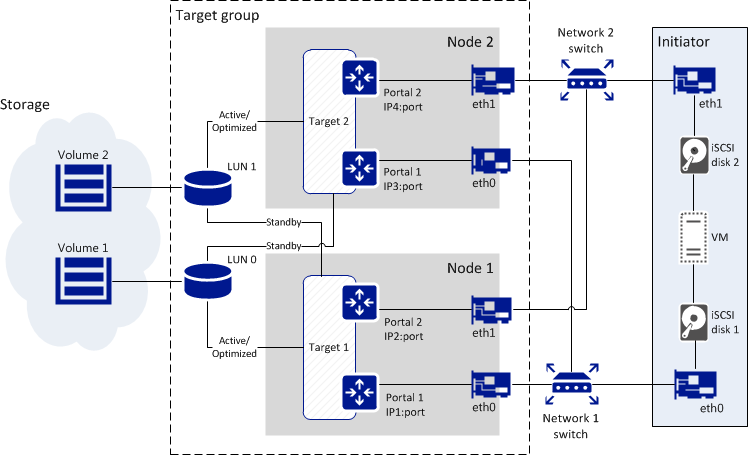
\includegraphics[width=\textwidth]{schema-iscsi.png}
    \caption{iSCSI protocol}
    \source{\href{https://dl.acronis.com/u/software-defined/html/AcronisCyberInfrastructure_3_5_admins_guide_en-US/exporting-storage/exporting-data-via-iscsi.html}{Exporting Storage via iSCSI}}
    \label{fig:icsci}
\end{figure}

CSI has been created to solve storage problematics for containerized workloads on Container Orchestration Systems (COs) like Kubernetes. It allows two actors, being the CO and the Storage Provider (SP), to interface together with the goal to provide storage where it is needed in the required quantity and size. The interface thus can be implemented as a CO or a SP.

The CO will be able to ask the SP to create a volume with a specified size, resize it, snapshot it, and eventually delete it. It can ask the SP to mount a volume on a specific host in order to make storage available for it. It allows to easily change the location of a certain volume, allowing it to move in coordination with containers using it across a cluster.
\color{black}

\subsection{iSCSI protocol}

\color{darkgreen}
iSCSI est une abréviation de Internet Small Computer System Interface. C'est un protocole réseau permettant d'émuler le fonctionnement du protocole SCSI, en transportant les commandes de ce protocole via un réseau IP. SCSI pour sa part est un standard définissant un bus informatique permettant de relier un ordinateur à un périphérique de stockage.
\color{black}

\subsection{General overview}

\color{darkgreen}
In summary, the CO (Kubernetes in this schema, but it can be any CO implementing CSI) send CSI commands to node and controller servers. The controller uses the dothill-api-go library to send API calls to the appliance to create and map volumes. Nodes then attach and mount mapped devices on the host using the csi-lib-iscsi library, and Kubernetes bind mount the mounted path in containers requiring a volume.
\color{black}

\begin{figure}[h]
    \centering
    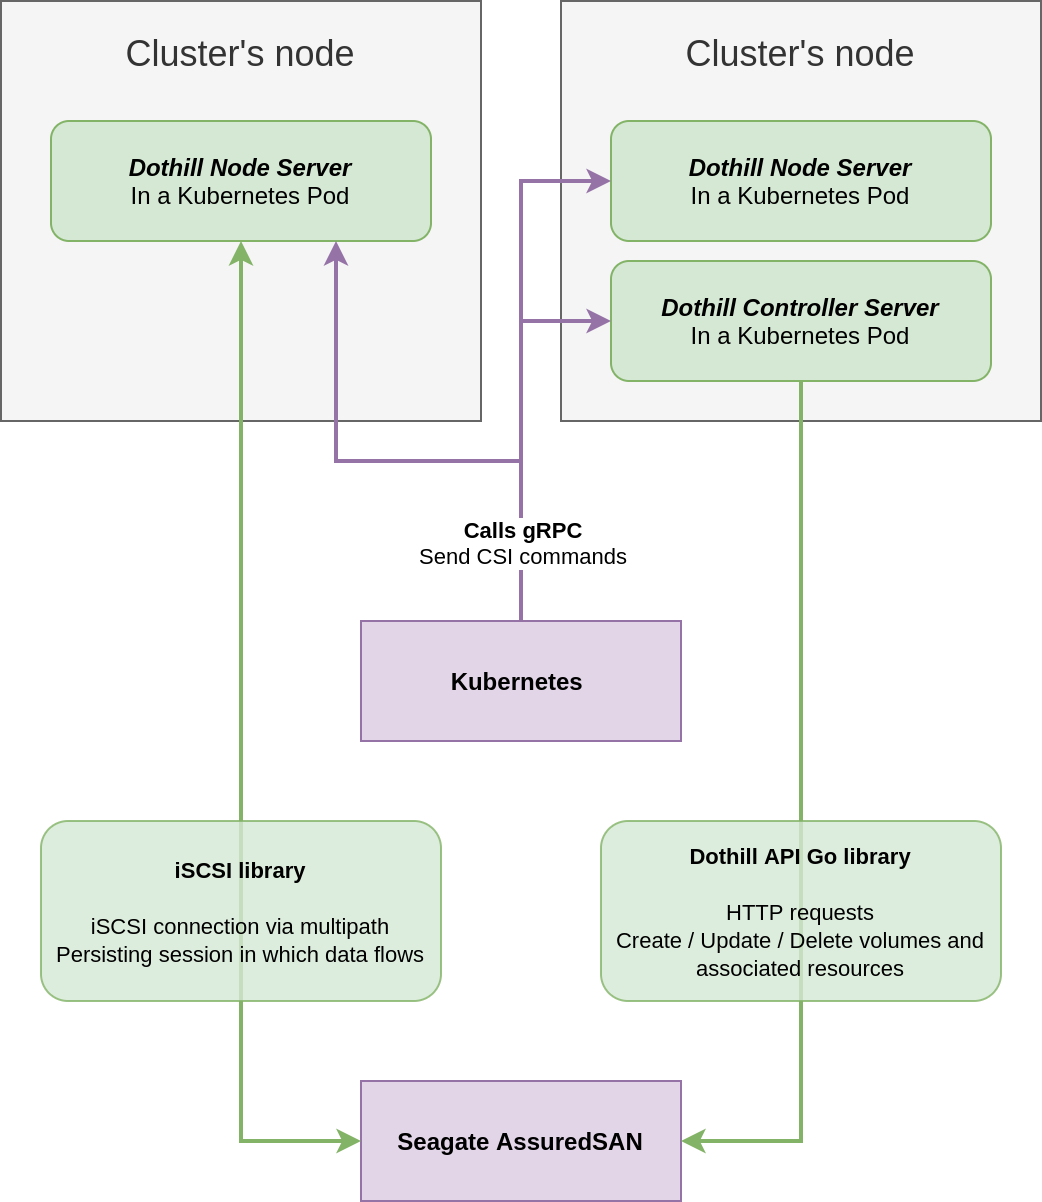
\includegraphics[width=10cm]{schema-san-iscsi-csi-simplified.png}
    \caption{Interactions between \glsdef{k8s} and \gls{san-iscsi-csi}}
    \label{fig:k8s-san-scsi-csi}
\end{figure}

\subsection{Difficulties encountered}

\color{darkgreen}
Using multipathd was very important to us to achieve high-availability. However we had some trouble using it, multipathd is operating at a quite low level thus it is not always easy to understand what is going on.

To ensure that our plugin is working perfectly smoothly, we tested it a lot, in many different use cases. The main issue we faced was filesystem corruption (which is a huge one). There are several cases in which multipathd can map devices in a way that can produce corruption or at least looks like a corruption. We fixed bugs one by one in order to ensure we have a fully corruption free driver.

// state that it is still not working perfectly.
\color{black}

\section{Work team}

\subsection{Context}

\subsection{Organization}

\clearpage
